% Fiche explicative : le power prior (chapitre 2, section 2.4)
% EPD-SDIA-4112 -- Statistique bayesienne (M1 SDIA)
% Toutes les valeurs numeriques proviennent de figures/key_numbers_ch2.json
% (scripts src/fig_ch2.py, verifiees par recalcul independant).
\documentclass[11pt,a4paper]{article}
\usepackage[french]{babel}
\usepackage{amsmath,amssymb}
\usepackage{booktabs}
\usepackage{graphicx}
\usepackage{xcolor}
\usepackage[most]{tcolorbox}
\usepackage[margin=1.9cm]{geometry}
\usepackage{enumitem}
\usepackage{titlesec}

\newcommand{\given}{\,\mid\,}
\newcommand{\data}{\mathbf{y}}
\newcommand{\N}{\mathcal{N}}

\definecolor{bleu}{HTML}{1F4E79}
\definecolor{gris}{HTML}{6B7280}
\definecolor{fondbox}{HTML}{F4F7FA}
\definecolor{orange}{HTML}{C2410C}

\titleformat{\section}{\normalfont\large\bfseries\color{bleu}}{\thesection.}{0.5em}{}
\titlespacing{\section}{0pt}{9pt}{4pt}
\setlist[itemize]{leftmargin=1.1em,itemsep=1.5pt,topsep=2pt,parsep=0pt}

\newtcolorbox{idee}{colback=fondbox,colframe=bleu,boxrule=0.4pt,arc=2pt,
  left=7pt,right=7pt,top=5pt,bottom=5pt,fonttitle=\bfseries,
  title={\small Idée clé}}
\newtcolorbox{piege}{colback=white,colframe=orange,boxrule=0.4pt,arc=2pt,
  left=7pt,right=7pt,top=5pt,bottom=5pt,fonttitle=\bfseries,
  title={\small Pièges à éviter}}

\sloppy
\setlength{\parindent}{0pt}
\setlength{\parskip}{4pt}

\begin{document}

\begin{center}
{\LARGE\bfseries\color{bleu} Le \emph{power prior}}\\[3pt]
{\large Régler le poids du passé quand l'historique contredit le présent}\\[5pt]
{\small\color{gris} EPD-SDIA-4112 --- Statistique bayésienne --- Chapitre 2, section 2.4 ---
Dr.\ Noulapeu Ngaffo Armielle}
\end{center}

\vspace{-2pt}
\hrule
\vspace{6pt}

\section{Le problème en une phrase}

Dans une étude, on dispose souvent d'un \textbf{résultat antérieur} (essai pilote,
littérature, registre) et de \textbf{données nouvelles}. Si le passé et le présent
\textbf{concordent}, on veut emprunter de la force au passé : plus de précision sans
refaire l'étude. S'ils \textbf{se contredisent}, un prior informatif classique impose
l'ancien résultat à des données qui le contredisent --- un mauvais service rendu à l'analyse.

Le \emph{power prior} répond à ce dilemme par un \textbf{seuil gradué} : au lieu de choisir
entre « ignorer l'historique » et « l'imposer entièrement », on \textbf{règle son poids}.

\begin{idee}
On élève la vraisemblance historique à une puissance $a_0 \in [0,1]$ :
\[
p(\theta) \;\propto\; p(\theta \given \data_0)^{\,a_0}
\]
$a_0 = 0$ : l'historique est \textbf{ignoré}. \quad
$a_0 = 1$ : il est pris \textbf{entier}. \quad
Entre les deux, un \textbf{curseur} --- et c'est là toute l'idée.
\end{idee}

\textbf{Pourquoi élever à une puissance, et non mettre un prior plus ou moins vague ?}
Parce que $a_0$ a une lecture directe : il agit comme un \textbf{compte d'essais}. Dans le
cas conjugué, $a_0(n_0 - s_0)$ et $a_0 s_0$ remplacent $(n_0-s_0)$ et $s_0$ : le passé ne
compte plus que pour $a_0 n_0$ observations. On parle de \textbf{taille d'échantillon
effective} (ESS) : $\text{ESS} = a_0 n_0 + n_1$. C'est un chiffre que l'on peut
\textbf{défendre}, chiffre en main, devant un comité ou un relecteur.

\section{L'exemple traité dans le cours}

Le cours déroule un conflit net, entièrement analytique (aucun échantillonnage requis) :

\begin{itemize}
  \item \textbf{Historique} : $s_0 = 20$ succès sur $n_0 = 100$ essais, soit $p_0 = 0{,}20$ ;
  \item \textbf{Étude actuelle} : $s_1 = 80$ succès sur $n_1 = 200$ essais, soit $p_1 = 0{,}40$.
\end{itemize}

Avec une vraisemblance binomiale et une loi Beta conjuguée, le posterior est
\[
\theta \given \data \;\sim\;
\mathrm{Beta}\bigl(\underbrace{a_0 s_0 + s_1 + 1}_{\alpha},\;\;
\underbrace{a_0 (n_0 - s_0) + (n_1 - s_1) + 1}_{\beta}\bigr),
\]
si bien que la moyenne a posteriori s'écrit
$\;\alpha/(\alpha+\beta)$ --- une fonction \emph{continue et décroissante} de $a_0$.

\begin{center}
\small
\resizebox{\linewidth}{!}{%
\begin{tabular}{@{}lcccc@{}}
\toprule
\textbf{Poids $a_0$} & \textbf{Données prises en compte} & \textbf{Taille effective} &
\textbf{Moyenne a posteriori} & \textbf{IC 95\,\%} \\
\midrule
$0$ \;\;(historique ignoré)      & actuelles seules            & $200$ & $0{,}4010$ & $[0{,}3346\,;0{,}4693]$ \\
$0{,}25$                          & $1/4$ de l'historique       & $225$ & $0{,}3789$ & $[0{,}3170\,;0{,}4428]$ \\
$0{,}50$                          & moitié de l'historique      & $250$ & $0{,}3611$ & $[0{,}3030\,;0{,}4213]$ \\
$0{,}75$                          & $3/4$ de l'historique       & $275$ & $0{,}3466$ & $[0{,}2917\,;0{,}4035]$ \\
$1$ \;\;(historique entier)       & historique $+$ actuel       & $300$ & $0{,}3344$ & $[0{,}2824\,;0{,}3886]$ \\
\bottomrule
\end{tabular}}
\end{center}

\begin{center}
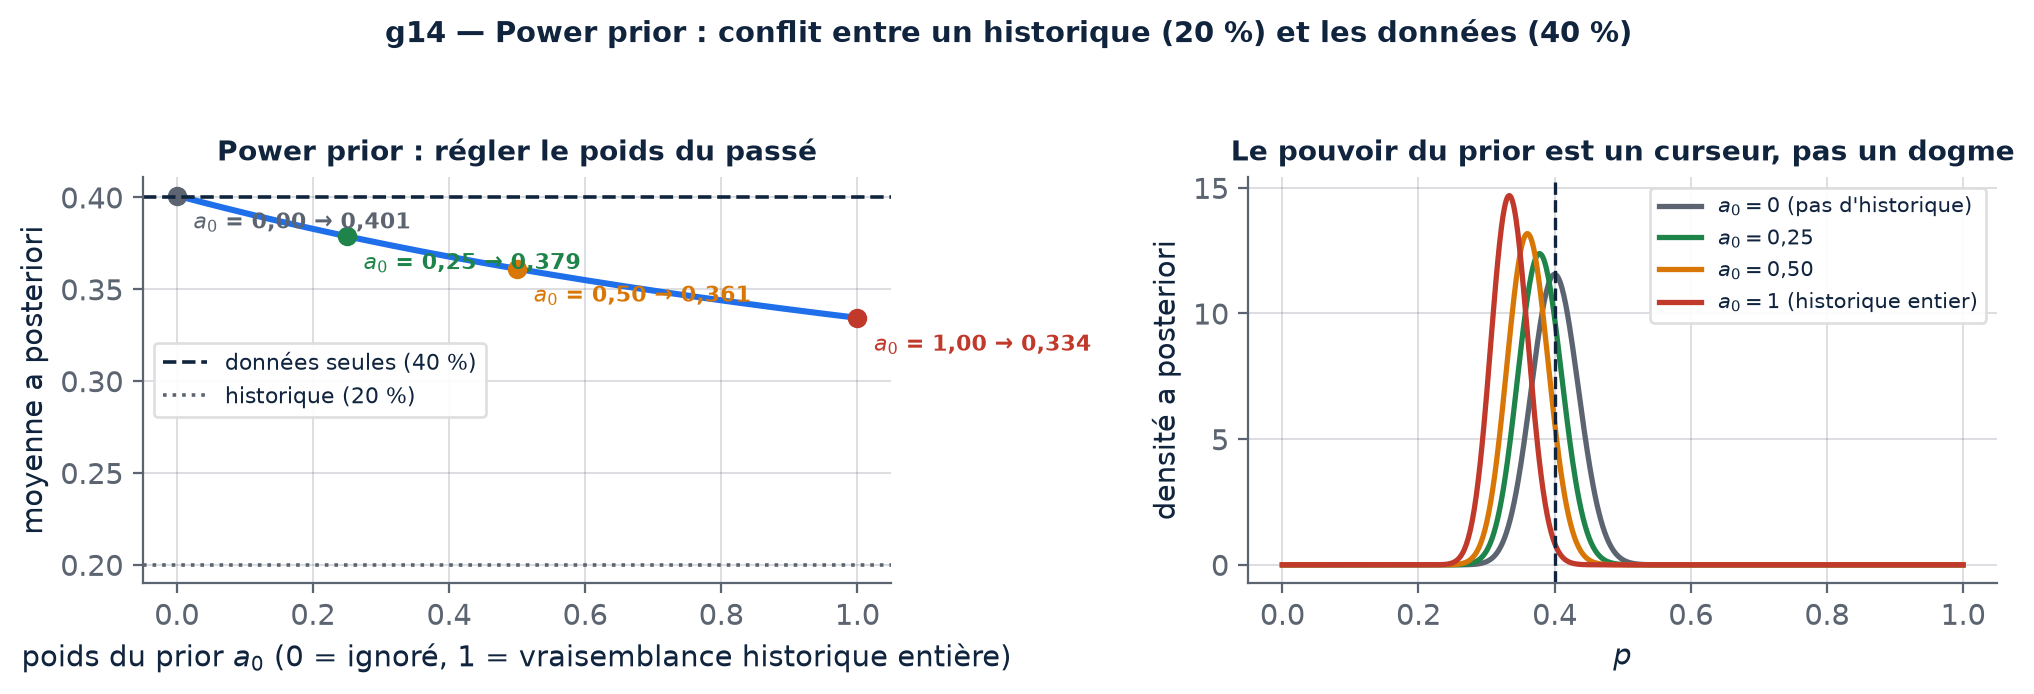
\includegraphics[width=0.86\textwidth]{g14_power_prior.png}
\end{center}

La lecture est immédiate : plus on emprunte au passé, plus l'estimation \textbf{tire vers
$0{,}20$} et plus l'intervalle se resserre. Avec $a_0 = 1$, la moyenne tombe à
$0{,}3344$ --- dont l'intervalle $[0{,}2824\,;0{,}3886]$ \textbf{exclut} le $0{,}40$
observé dans l'étude actuelle. Voilà précisément ce que l'on veut rendre visible et
discutable : \emph{le prix, en biais, de la confiance accordée au passé}.

\section{Comment choisir $a_0$}

\begin{itemize}
  \item \textbf{Jamais après avoir vu le résultat.} $a_0$ se fixe \textbf{avant} l'analyse et
        se justifie par des arguments cliniques ou méthodologiques (qualité, ancienneté,
        transposabilité de l'étude source).
  \item \textbf{Par la taille effective.} On raisonne souvent ainsi : « je veux que le passé
        pèse environ la moitié d'un bras d'essai », ce qui détermine $a_0$ à partir de $n_0$.
  \item \textbf{En rapportant la sensibilité.} La bonne pratique est de présenter
        \textbf{plusieurs valeurs} de $a_0$ (une courbe, comme ci-dessus) plutôt qu'une seule,
        afin que le lecteur voie la dépendance du résultat à l'hypothèse.
  \item \textbf{Comme un paramètre à part entière.} Le désaccord passé/présent devient
        un \emph{paramètre} que la discussion scientifique peut traiter explicitement,
        au lieu d'être enfoui dans un choix de prior.
\end{itemize}

\begin{piege}
\textbf{« $a_0 = 1$ est le choix objectif, puisque l'historique est de bonne qualité. »}\\
C'est faux : $a_0 = 1$ revient à traiter les $100$ observations du passé comme si elles
avaient été collectées dans l'étude actuelle, avec le même protocole et la même population.
Le power prior existe justement parce que ce n'est \textbf{pas} exactement le cas.\\[2pt]
\textbf{« Un prior vague règle le problème. »}\\
Il noie seulement le conflit : avec un prior vague, on n'emprunte rien, donc on perd le
bénéfice de la précision --- et on ne dit rien du désaccord. Le power prior, lui, le
\textbf{chiffre}.\\[2pt]
\textbf{Attention à la formulation.} $p(\theta) \propto p(\theta \given \data_0)^{a_0}$
n'est un \emph{vrai} prior que pour un historique fixé ; dans les variantes où $a_0$ est
estimé sur les données, il devient un paramètre de plus et la normalisation doit être
traitée rigoureusement.
\end{piege}

\section{Où cela s'articule dans le cours}

\begin{itemize}
  \item \textbf{Section 2.4} (« Combien de données pour effacer un prior ? ») : le power
        prior est l'une des trois réponses du chapitre, avec la hiérarchie et la courbe
        de sensibilité.
  \item \textbf{Lien avec la section 2.3} : c'est le traitement rigoureux du
        \emph{désaccord} entre un prior et les données, là où l'analyse de sensibilité
        se contente de constater le conflit.
  \item \textbf{Lien avec le chapitre 4} : la même question réapparaît sous forme de
        facteur de Bayes et de poids de modèles.
  \item \textbf{Lien avec le chapitre 5} : le prior hiérarchique (pooling partiel) est
        l'approche moderne du même problème quand on dispose de \emph{plusieurs}
        historiques au lieu d'un seul.
  \item \textbf{Travaux pratiques} : le notebook du chapitre
        \texttt{TP2\_a\_priori\_}\allowbreak\texttt{a\_posteriori.ipynb}, et le mini-projet
        radon \texttt{Mini-projet-modele-}\allowbreak\texttt{hierarchique-radon}.
\end{itemize}

\enlargethispage{3\baselineskip}
\vspace{4pt}
{\footnotesize\color{gris}
Source des chiffres : \texttt{figures/key\_numbers\_ch2.json}, produits par
\texttt{src/fig\_ch2.py} (figure \texttt{g14\_power\_prior.png}) et vérifiés par recalcul
indépendant. Reproduire : \texttt{python src/fig\_ch2.py} puis
\texttt{python src/build.py}.}

\end{document}
